% estcj.py

\documentclass[landscape,12pt,a4paper]{article}
\usepackage[body={24cm,17cm}]{geometry}
\usepackage{hyperref}
\hypersetup{colorlinks=true,linkcolor=blue}
\usepackage{graphicx}
\usepackage{listings}
\lstset{basicstyle=\footnotesize\ttfamily, showstringspaces=false, identifierstyle=, keywordstyle=}
\lstset{numbers=left, numberstyle=\tiny, stepnumber=1, numbersep=5pt, frame=single}
\lstset{language={}, breaklines=true}

%------------------------------------------------------------------
% a couple horizontal bars to delimit embedded code
% the width suits that set above and
% the mathmode eliminates spaces between the three elements
\newcommand{\topbar}{\ensuremath{
    \rule{0.1mm}{2.0mm} \rule[2.0mm]{239.5mm}{0.1mm} \rule{0.1mm}{2.0mm}
}}
\newcommand{\bottombar}{\ensuremath{
    \rule{0.1mm}{2.0mm} \rule{239.5mm}{0.1mm} \rule{0.1mm}{2.0mm}
}}


%------------------------------------------------------------------
% Title page information
%------------------------------------------------------------------

\title{
  Estimation of high-enthalpy flow conditions
  for simple shock and expansion processes using
  the ESTCj program and library.
}
\author{
  Mechanical Engineering Report 2011/02 \\
  P.~A.~Jacobs, R.~J.~Gollan, D.~F.~Potter, F.~Zander,\\
  D.~E.~Gildfind, P.~Blyton, W.~Y.~K.~Chan and L.~Doherty \\
  Centre for Hypersonics\\
  The University of Queensland
}

\begin{document}
\maketitle

\baselineskip = 1.2pc

\begin{abstract}
This report presents the software tools that we have built to do simple
flow process calculations for ideal gases and gases in chemical equilibrium.
The software comes in the form of a library for the most fundamental processes and
an application program, ESTCj, for convenient calculation of 
the combined flow processes relevant to shock- and expansion-tube operation.
\end{abstract}

\newpage
\tableofcontents

%------------------------------------------------------------------

\newpage
\section{Introduction}
%
ESTCj\,\footnote{Equilibrium Shock Tube Conditions, junior} 
began as a re-implementation of the ideas in the ESTC code\,\cite{mcintosh_70}
written by Malcolm McIntosh in the late 1960s and 
the shock-tube-plus-nozzle (STN) code\,\cite{krek_jacobs_93} written in the early 1990s.
The new program\,\cite{jacobs_gardner_2003a} was started 
while PJ was on study leave at DLR Goettingen,
with a decision to delegate the equilibrium thermochemistry issues to the 
Gordon and McBride's Chemical Equilibrium Analysis (CEA) 
code\,\cite{gordon_mcbride_1994,mcbride_gordon_1996}.
With the thermochemistry provided by CEA, the ESTCj program had to be concerned
only with the smaller task of computing the flow changes across shocks and through
the steady nozzle expansion.

\medskip
Implementation was done in the Python programming language\,\footnote{http://www.python.org}
which was easy for end users to customize so the program tended to grow in an ad-hoc fashion.
This report describes the current generation of the program, which has been refactored into
three layers:
\begin{enumerate}
 \item Thermochemical gas models for perfect gases and gases in thermochemical equilibrium.
  Appendix\,\ref{gas-model-sec}.
 \item A library of functions for simple flow processes such as normal shocks, oblique shocks,
  and steady and unsteady expansions. Appendix\,\ref{process-code-sec}.
 \item A top-level code (actually called estcj.py) that coordinates the calling 
  of the flow-process functions using information provided by the user on the command line.
  Appendix\,\ref{estcj-py}.
\end{enumerate}
One of the advantages of moving the flow-process calculations to a library is that 
they can be conveniently reused, 
as has been done for the NENZFr code\,\cite{doherty_etal_2012a}, for example.
Three simple examples of building specific programs with the library are shown in
Section\,\ref{the-libraries}.

\medskip
The following sections provide an overview of the use of the new functions and their capabilities.
This is done mostly by way of examples.
The bulk of the detail is in the source code which we've tried to make modular and very readable.
Despite the code being central to this report, we have put it in the Appendix so that there is
a reasonable chance that the reader might at least get the overview 
before being overwhelmed by detail and giving up.

\newpage
\section{Operation of the ESTCj program}
%
The application-level code is essentially a command-line interpreter
that writes the results of the requested calculation to the standard-output stream
by default.
It's easiest to get a reminder of the available settings by asking for ``help''
on the command line.

\lstinputlisting[]{../notes/estcj-help.txt}

The default supporting gas model library (Appendix~\ref{cea2-gas-py}) calls upon the NASA Glenn CEA2 program 
for evaluation of the equilibrium thermochemical properties of gas mixtures.
The list of available gases in \verb!ESTCj! can be seen by using the \verb!--list-gas-names! option 
on the command line.
The list reflects the typical needs of the UQ shock and expansion tunnel operation but 
it is easy to add new gases to the \verb!make_gas_from_name()! function in the gas model code.

\bigskip
\subsection{Example of use for T4 condition}
%
Built into ESTCj is an idealized model of a reflected shock tube.
This model is composed of quasi-one-dimensional wave processes 
as shown in the following figure that has been taken from Ref.\,\cite{krek_jacobs_93}.
The numbers denote states of the gases between processes.

\begin{center}
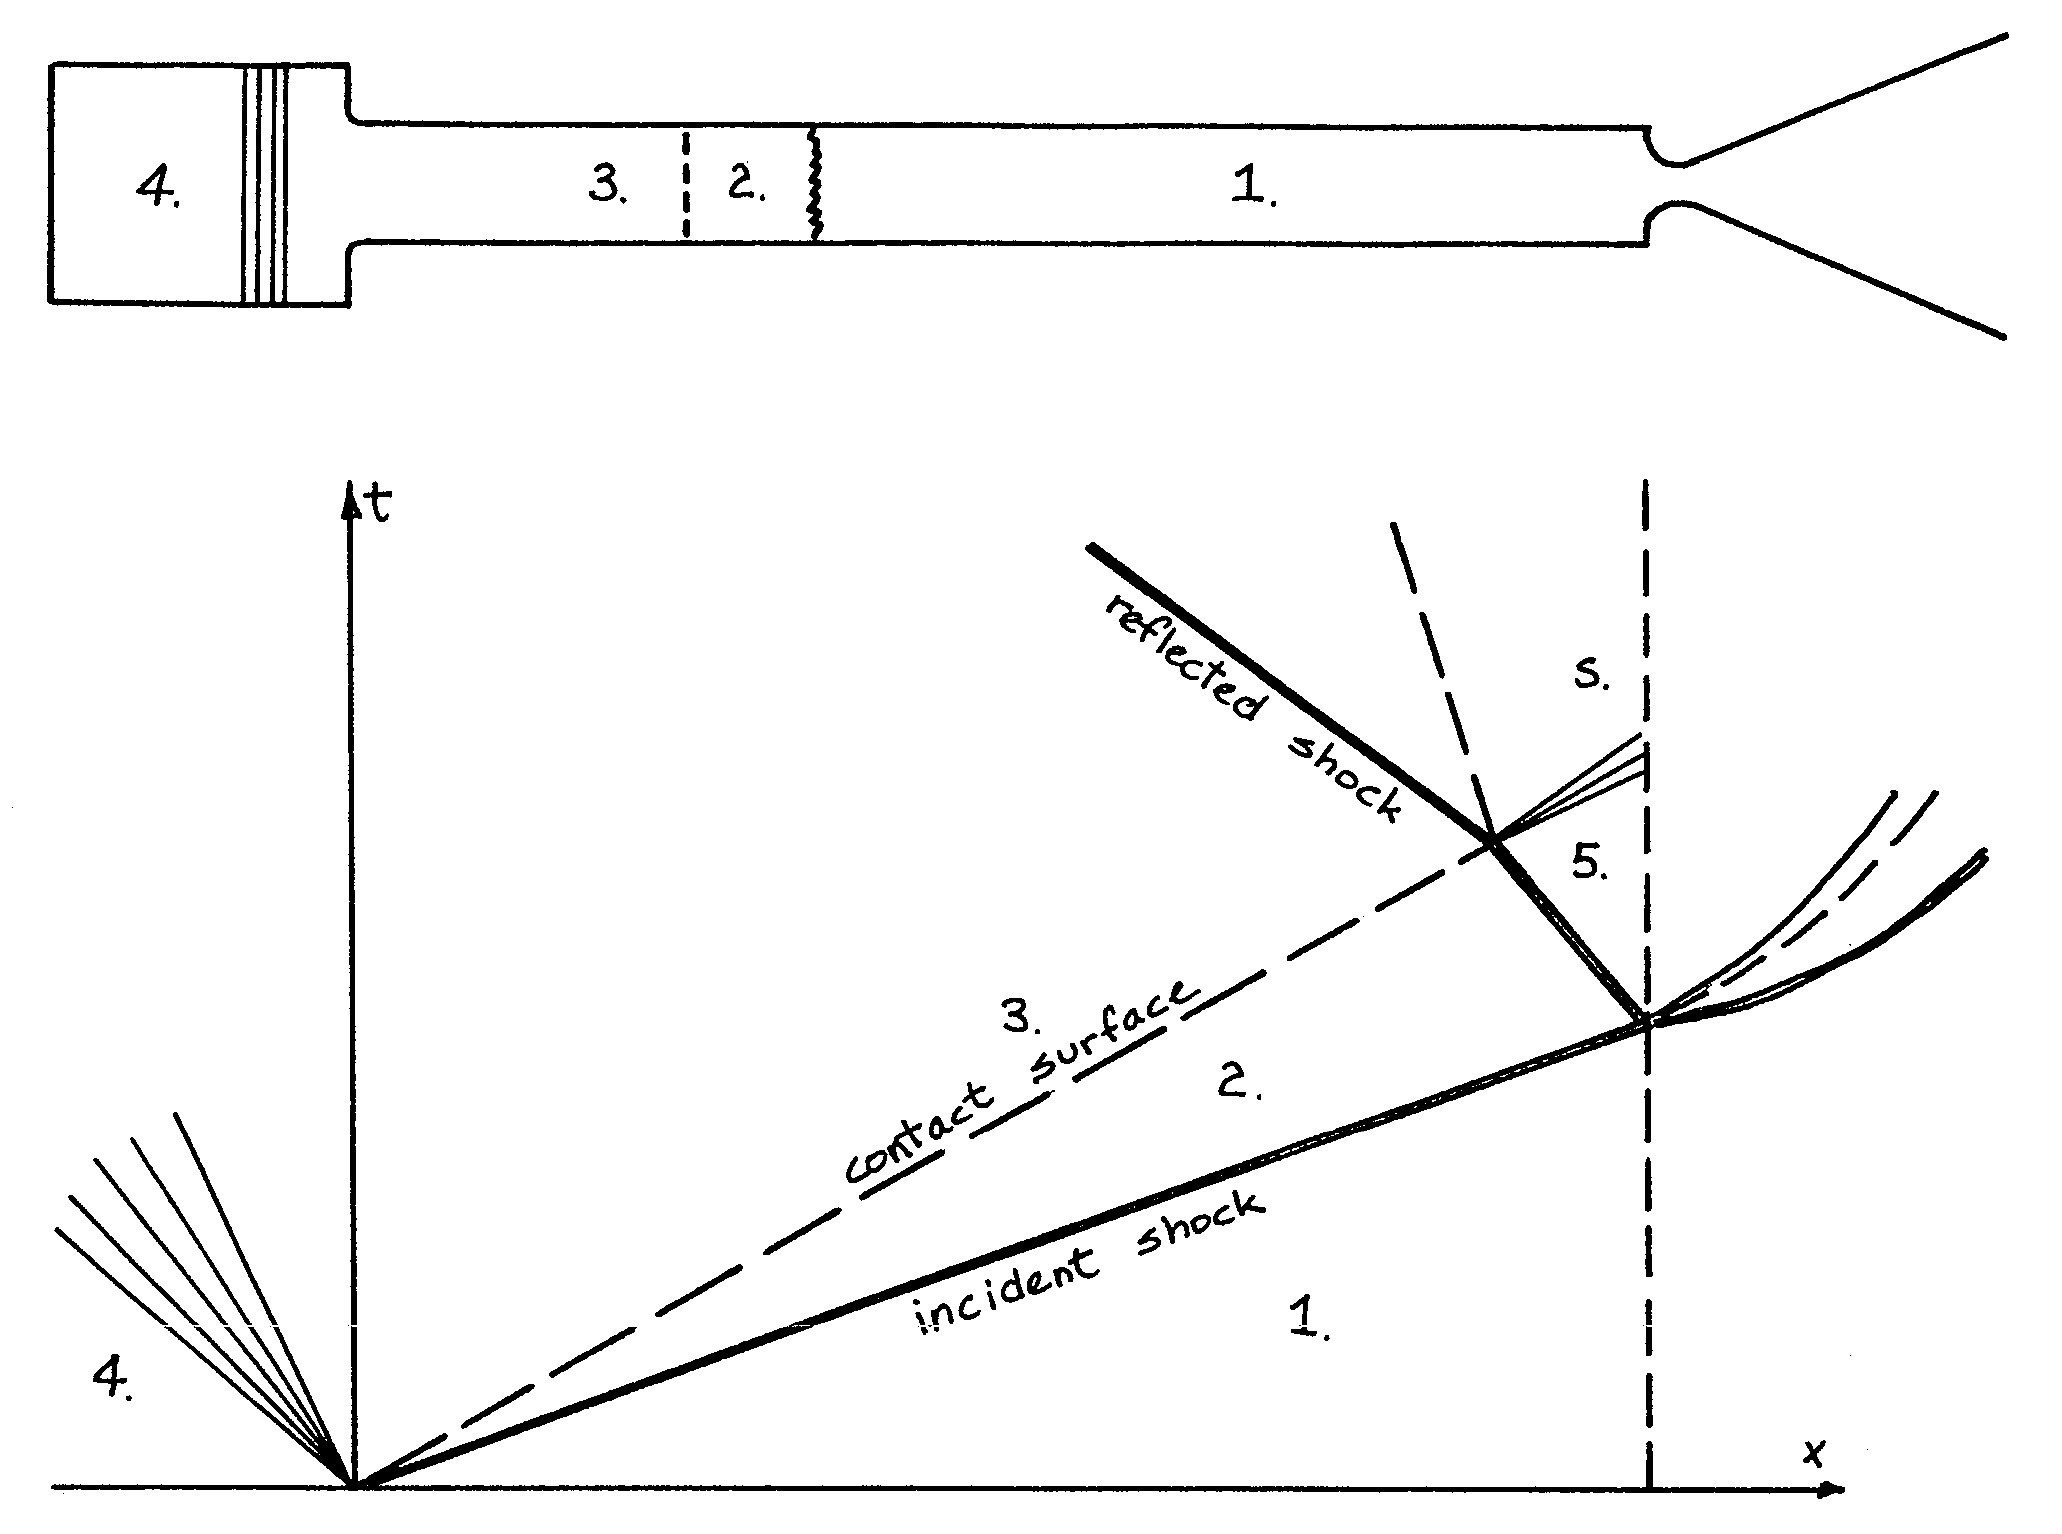
\includegraphics[width=10cm]{../figs/shock-tube-process-fig-from-stn-report.png}
\end{center}

\medskip
A typical low-enthalpy flow condition for the T4 shock tunnel may start with
a test gas (air) at room temperature ($T_1$ = 300\,K) 
and a little above atmospheric pressure ($p_1$ = 125\,kPa).
The observed shock speed, $V_s$, was 2414\,m/s and the observed nozzle-supply pressure
relaxed to 34.37\,MPa.
With the Mach 4 nozzle having an area ratio of 27, the flow conditions in the facility
may be computed using the command:
\begin{verbatim}
$ estcj.py --task=stn --gas=air --T1=300 --p1=125.0e3 --Vs=2414 --pe=34.37e6 --ar=27.0
\end{verbatim}
The full output is included below, where you should see that
this condition has an enthalpy of ($H_{5a} - H_1)$~=~5.43\,MJ/kg and the nozzle-exit condition
has a pressure of $P_7$~=~93.6\,kPa and a static temperature of $T_7$~=~1284\,K,
with a flow speed of $V_7$ = 2.95\,km/s.
Note that we have selected to stop the expansion at a particular nozzle area ratio.
Alternatively, we may stop the expansion at a particular Pitot pressure by specifying
\verb?--task=stnp? and a suitable ratio for the option \verb?--pp_on_pe?.
If you don't want to specify a relaxation pressure with option \verb?--pe?,
the reflected-shock conditions (5) will be used directly as the nozzle supply conditions.

\lstinputlisting[]{../notes/t4-condition-transcript.txt}

\medskip
By default, the \verb!cea2_gas! model is used, however, the CEA2 program can occasionally fail
to provide data at conditions of interest so the \verb!libgas_gas! module is provided 
as an alternative gas model.
This \verb!libgas! module is that used in the \verb!Eilmer3! code and may model the gas 
thermochemistry via look-up table data that has previously been generated by the CEA2 program. 
Here is the same T4 condition computed with a look-up table describing the air gas model.

\lstinputlisting[]{../notes/t4-condition-transcript-libgas.txt}

Note that there are some differences in computed detail.  
The look-up table was generated for temperatures higher than the initial shock tube 
fill temperature and the thermochemical model is using extrapolated parameter values 
for some of the calculation.

\subsection{Subset calculations}
%
Subset calculations of the shock-tube flow processing can be done by selecting a different task.
For example, just the incident shock processing can be computed with the \verb?--task=ishock?,
specifying only the gas, initial pressure, temperature and incident shock speed.
Here is an example from Huber's \cite{huber_1963a} Table IV for a speed of 37.06\,ft/s 
at a geopotential altitude of 173500\,feet.
The expected pressure (from Table IV) is 86.5\,kPa and the temperature is 12000\,K,
quite close to the values computed by \verb!ESTCj! and shown below.

\lstinputlisting[]{../notes/incident-shock-huber.txt}

This equilibrium-chemistry result can be compared with the ideal gas calculation 
for the same speed and free-stream condition.

\lstinputlisting[]{../notes/incident-shock-huber-ideal.txt}

\medskip
The following sections show the subproblems that can be exercised from the command line.
These calculations can also be done inside other programs by calling 
the relevant \verb?gas_flow.py? functions.

\bigskip
\subsection{Pitot pressure calculation}
%
Using the test flow conditions from the exit of the Mach 4 nozzle, we can then
compute the expected Pitot pressure to be 2.14\,MPa.

\lstinputlisting[]{../notes/pitot-transcript.txt}

\bigskip
\subsection{Cone surface pressure calculation}
%
Alternatively, the conditions on the surface of a conical pressure probe
(with 15$^o$ half-angle) can be computed as:

\lstinputlisting[]{../notes/cone-x3-transcript.txt}

\bigskip
\subsection{Total condition calculation}
%
The hypothetical stagnation conditions for a specified free stream
can be computed as:

\lstinputlisting[]{../notes/total-transcript.txt}

\newpage
\section{Building custom application with the supporting libraries}
\label{the-libraries}
%
Although the ESTCj is built specifically to do the calculations 
needed for flow conditions typical of the T4 reflected shock tunnel,
the supporting libraries are more general.
There are gas modules for:
\begin{itemize}
 \item a perfect gas, with user specified properties (Appendix\,\ref{ideal-gas-py}).
 \item a mixture of gases in thermochemical equilibrium (Appendix\,\ref{cea2-gas-py}).
   This module delegates calculation to the CEA2 code.
 \item the same gas models that are used in the L1d3 and Eilmer3 codes,
   but with chemical reactions omitted (Appendix\,\ref{libgas-gas-py}).
\end{itemize}
%
The flow process modules cover simple processes associated with:
\begin{itemize}
 \item normal shocks for one-dimensional flow.
 \item finite (isentropic) waves for one-dimensional flow.
 \item steady quasi-one-dimensional flow with area change.
 \item oblique shocks for planar and conical flow.
\end{itemize}
There is a module (Appendix\,\ref{ideal-gas-flow-py})
that assumes an ideal gas model and is very much an implementation of the classic
textbook gas-dynamic equations.
When using this module, the user needs to specify the
relevant gas properties (such as the ratio of specific heats).
The second flow process module (Appendix\,\ref{gas-flow-py}) uses \verb!Gas! objects
created by the cea2, libgas and ideal gas modules of Appendix\,\ref{gas-model-sec} 
and so can compute flow processes for a gas with the species in chemical equilibrium or frozen.

\medskip
There are many ways these functions can be combined, however,
this section is deliberately terse because the codes in the appendices are well documented
and follow the standard texts on gas dynamics.
The only unusual formulation is that for the Taylor-Maccoll flow with the general gas model.
For that formulation, the notes from PJ's workbook are included 
in Appendix\,\ref{pj-notes-cone-flow}.


\bigskip
\subsection{Oblique shock for air in chemical equilibrium}
%
Hunt and Sounders\,\cite{hunt_souders_1975a} provide tabulated data for the processing
of air in chemical equilibrium by oblique shocks.
Here are a couple of examples of calling up the \verb!gas_flow! functions to do the same job
with a \verb!cea2_gas! object.

\lstinputlisting[]{../notes/oblique_shock_example.py}

\lstinputlisting[]{../notes/oblique_shock_example_transcript.txt}


\subsection{Classic shock tube}
%
As an example of building a custom application, consider the idealized shock tube 
with equal area sections separated by a diaphragm.
State 1 is air at low pressure on the downstream-side of a diaphragm and 
state 4 is high pressure helium initially on the upstream side of the diaphragm.
When the diaphragm is removed (ideally), the helium expands into the part of the tube
occupied initially by the air and drives a shock through the quiescent air.
State 2 is the shock-compressed air and state 3 is the expanded helium
driving the air.
At the moving contact surface between the air and helium, the pressures and velocities
of the air and helium have to match.
See for example, Section 7.8 (Shock tube relations) in Anderson's text\,\cite{anderson_82}
for a discussion based on perfect gas behaviour.

\medskip
The example code sets up a function that, given the pressure at the contact surface,
returns the difference in velocities of the gases at the contact surface.
This function is passed to a nonlinear equation solver to determine the pressure ratio
at which the velocity difference is zero.
All of the interesting calculation, 
along with the printing of the computed states, is done by line 60.
The next 40 lines (approximately) of the script write out the flow data in small steps, 
so that they may be used for comparison with data from a CFD calculation.

\lstinputlisting[]{../../../eilmer3/2D/classic-shock-tube/classic_shock_tube.py}

\bigskip
\subsection{Idealized expansion tube}
%
As a second example of building a custom application, consider the idealized expansion
of the test gas in an expansion tube\,\cite{trimpi_62}.
We will include just the processing of the test gas by the incident shock,
followed by the unsteady expansion to test-section conditions. 
The states in the calculation are:
\begin{itemize}
 \item [1.] Initial (quiescent) test gas, filling the shock tube.
 \item [2.] Shock-processed test gas.
 \item [5.] Expanded test gas, as would be expected to emerge from the downstream-end of the acceleration tube.
 \item [10.] Initial accelerator gas, filling the acceleration tube, downstream of the shock tube.
 \item [20.] Shock-processed accelerator gas that is pushed along, in front of the expanded test gas.
\end{itemize}
The final expansion process is regulated by the fill pressure of the acceleration tube
and the test-gas conditions are determined by balancing the expanded gas pressure against
the post shock pressure of the acceleration gas.
When computing this balance iteratively, we guess the pressure and compute the two velocities.
As done in the classic shock-tube example, 
we use the difference between the two velocities as the measure of error for the guessed pressure.



\lstinputlisting[]{../../../../lib/cfpylib/gasdyn/classic_expansion_tube.py}

%------------------------------------------------------------------

\newpage
\bibliographystyle{unsrt}
\bibliography{../bibtex/pj,../bibtex/shocktube,../bibtex/gas,../bibtex/gas_dynamic.bib}

%--------------------------------------------------------------------
% Appendices
%--------------------------------------------------------------------

\newpage
\appendix
\section{Source code for gas models}
\label{gas-model-sec}
%
\subsection{ideal\_gas.py}
\label{ideal-gas-py}
%
Thermodynamic functions for an ideal gas.

\lstinputlisting[language={}]{../../../../lib/cfpylib/gasdyn/ideal_gas.py}

\newpage
\subsection{libgas\_gas.py}
\label{libgas-gas-py}
%
Thermodynamic functions for the gas model used by Eilmer3.

\lstinputlisting[language={}]{../../../../lib/cfpylib/gasdyn/libgas_gas.py}

\newpage
\subsection{cea2\_gas.py}
\label{cea2-gas-py}
%
Thermodynamic functions for the thermochemical-equilibrium gas model backed by CEA2.

\lstinputlisting[language={}]{../../../../lib/cfpylib/gasdyn/cea2_gas.py}

\newpage
\section{Source code for flow process calculations}
\label{process-code-sec}
%
\subsection{ideal\_gas\_flow.py}
\label{ideal-gas-flow-py}
%
Basic flow relations for an ideal gas.

\lstinputlisting[language={}]{../../../../lib/cfpylib/gasdyn/ideal_gas_flow.py}

\newpage
\subsection{gas\_flow.py}
\label{gas-flow-py}
%
Basic flow relations for a more general gas.

\lstinputlisting[language={}]{../../../../lib/cfpylib/gasdyn/gas_flow.py}

\newpage
\section{Source code for ESTCj application}
\label{estcj-py}
%
Top-level application code.

\lstinputlisting[language={}]{../../../../app/nenzfr/estcj.py}

\newpage
\section{Notes on conical flow}
\label{pj-notes-cone-flow}
%
Scanned straight from PJ's workbook, warts and all.

\begin{center}
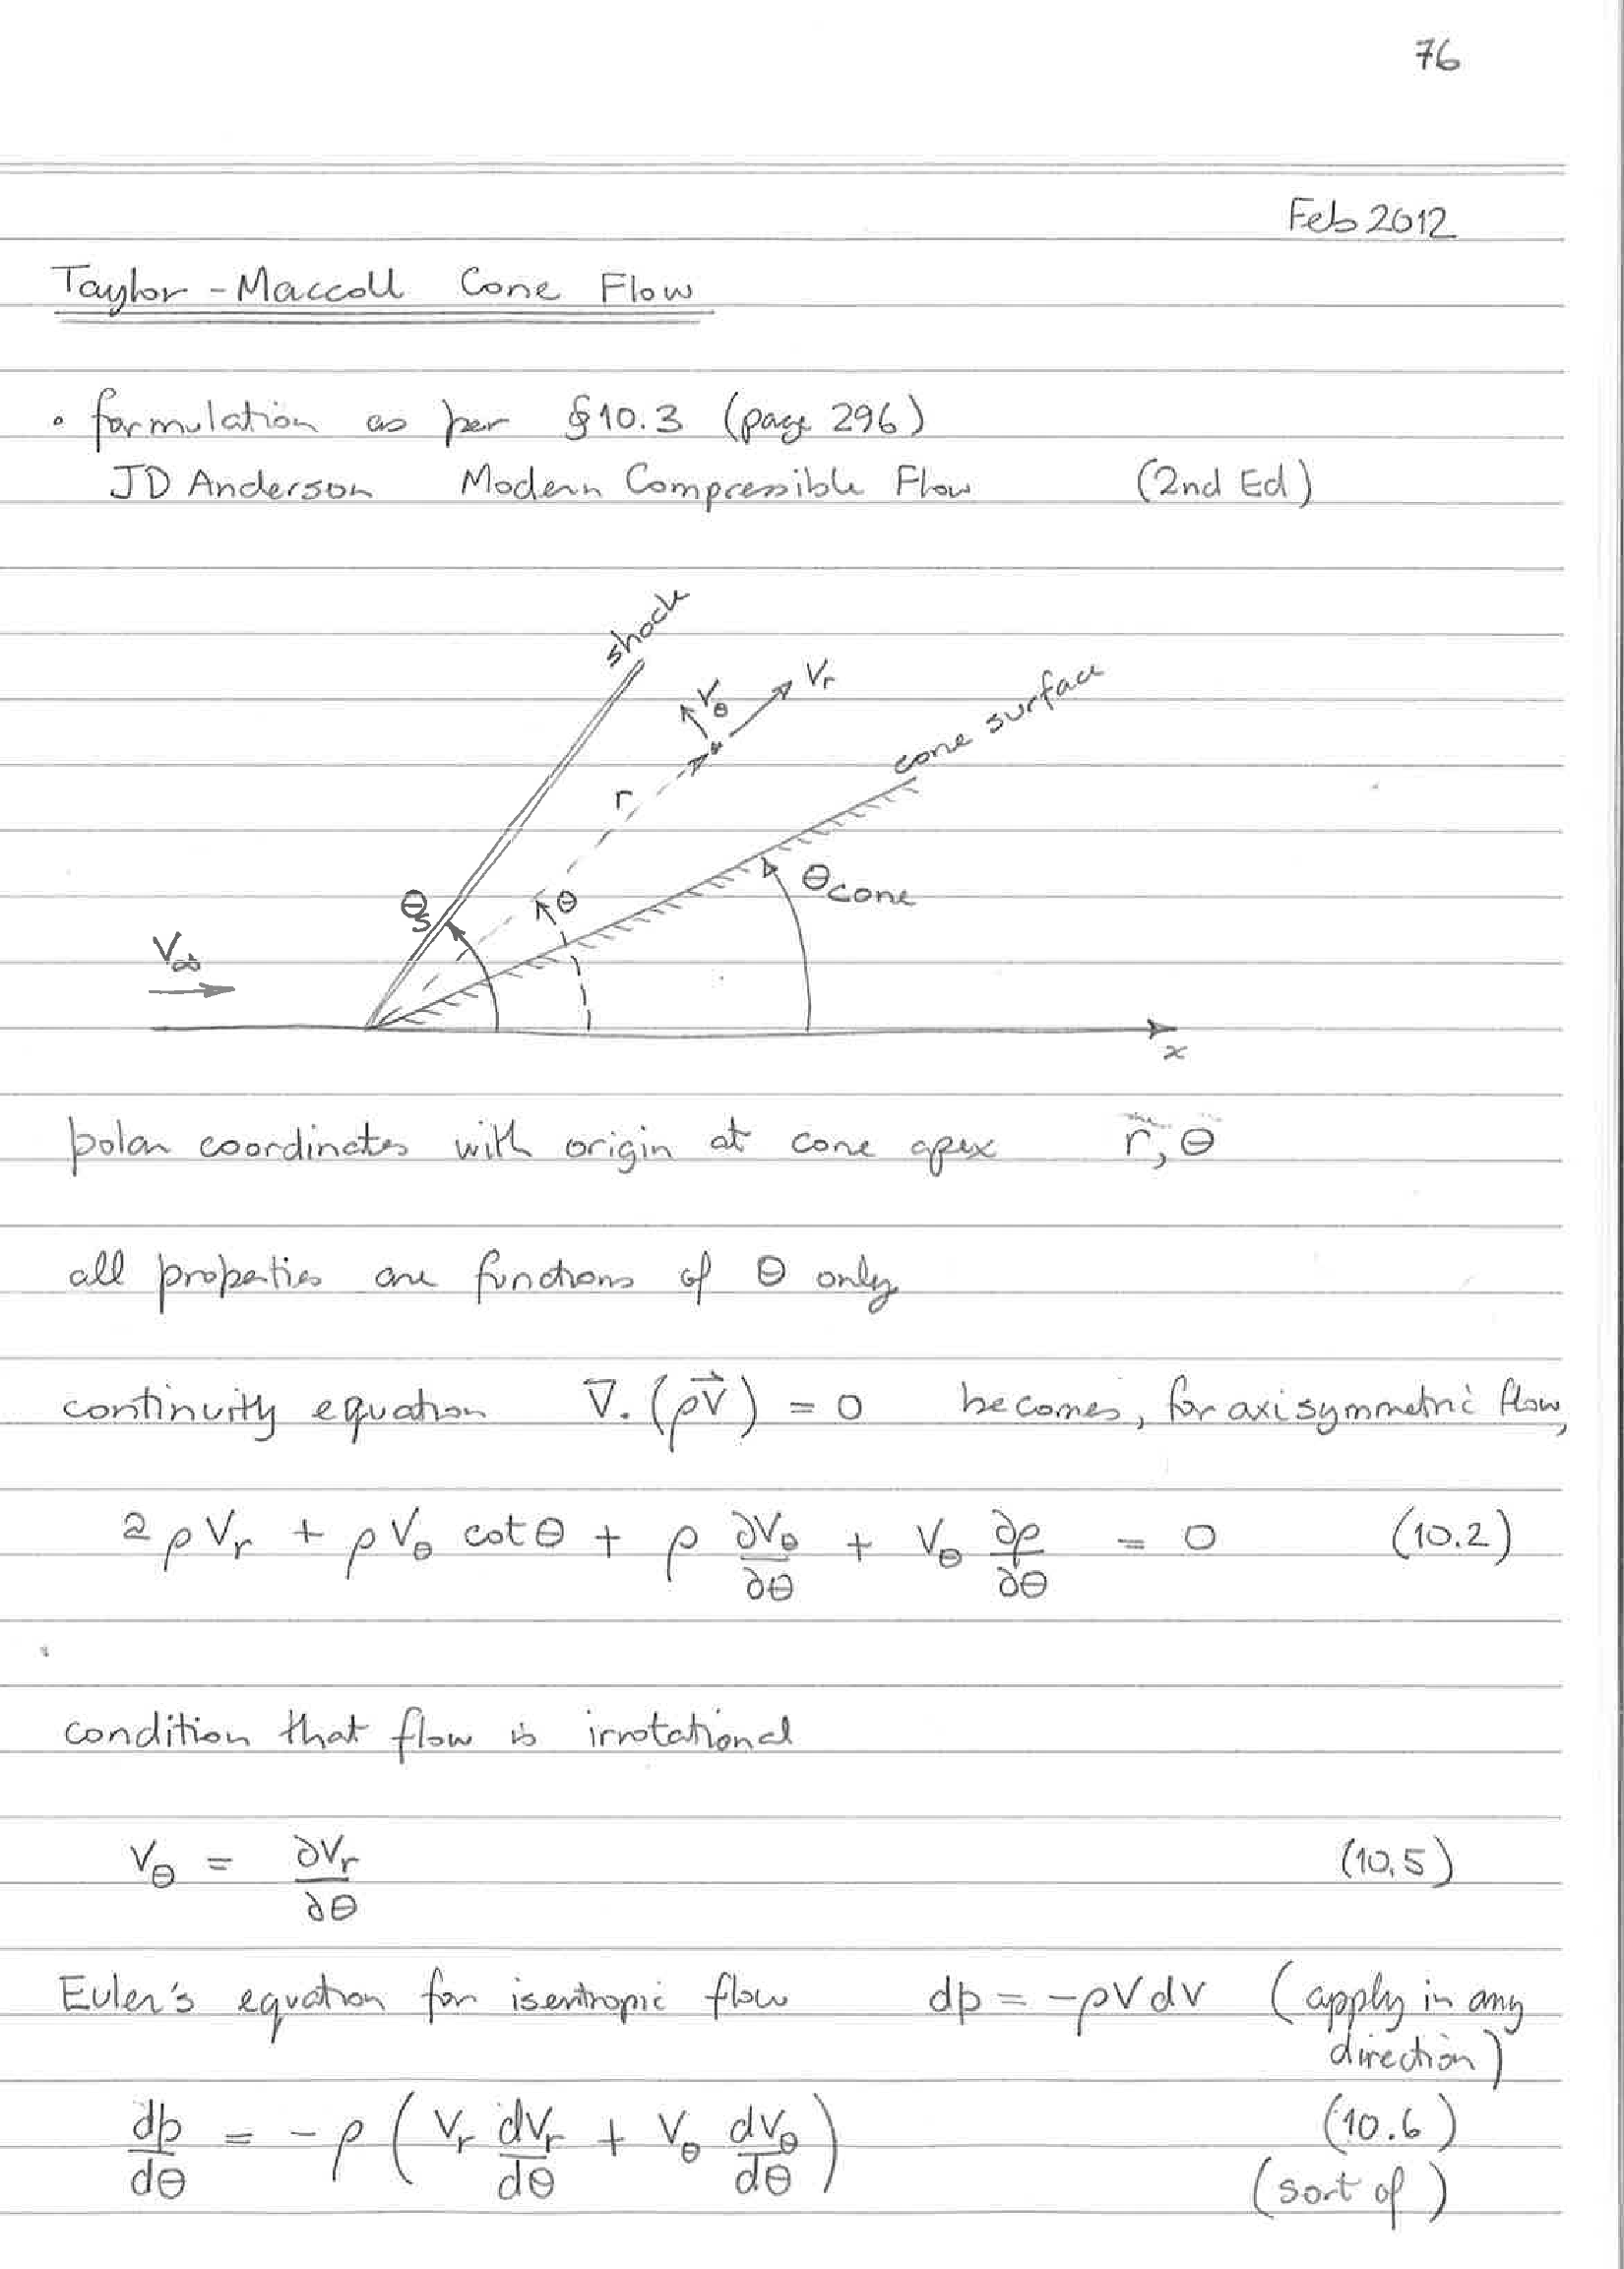
\includegraphics[width=0.9\textheight,angle=90]{../figs/pj-workbook-page-76.png}
\end{center}

\newpage
\begin{center}
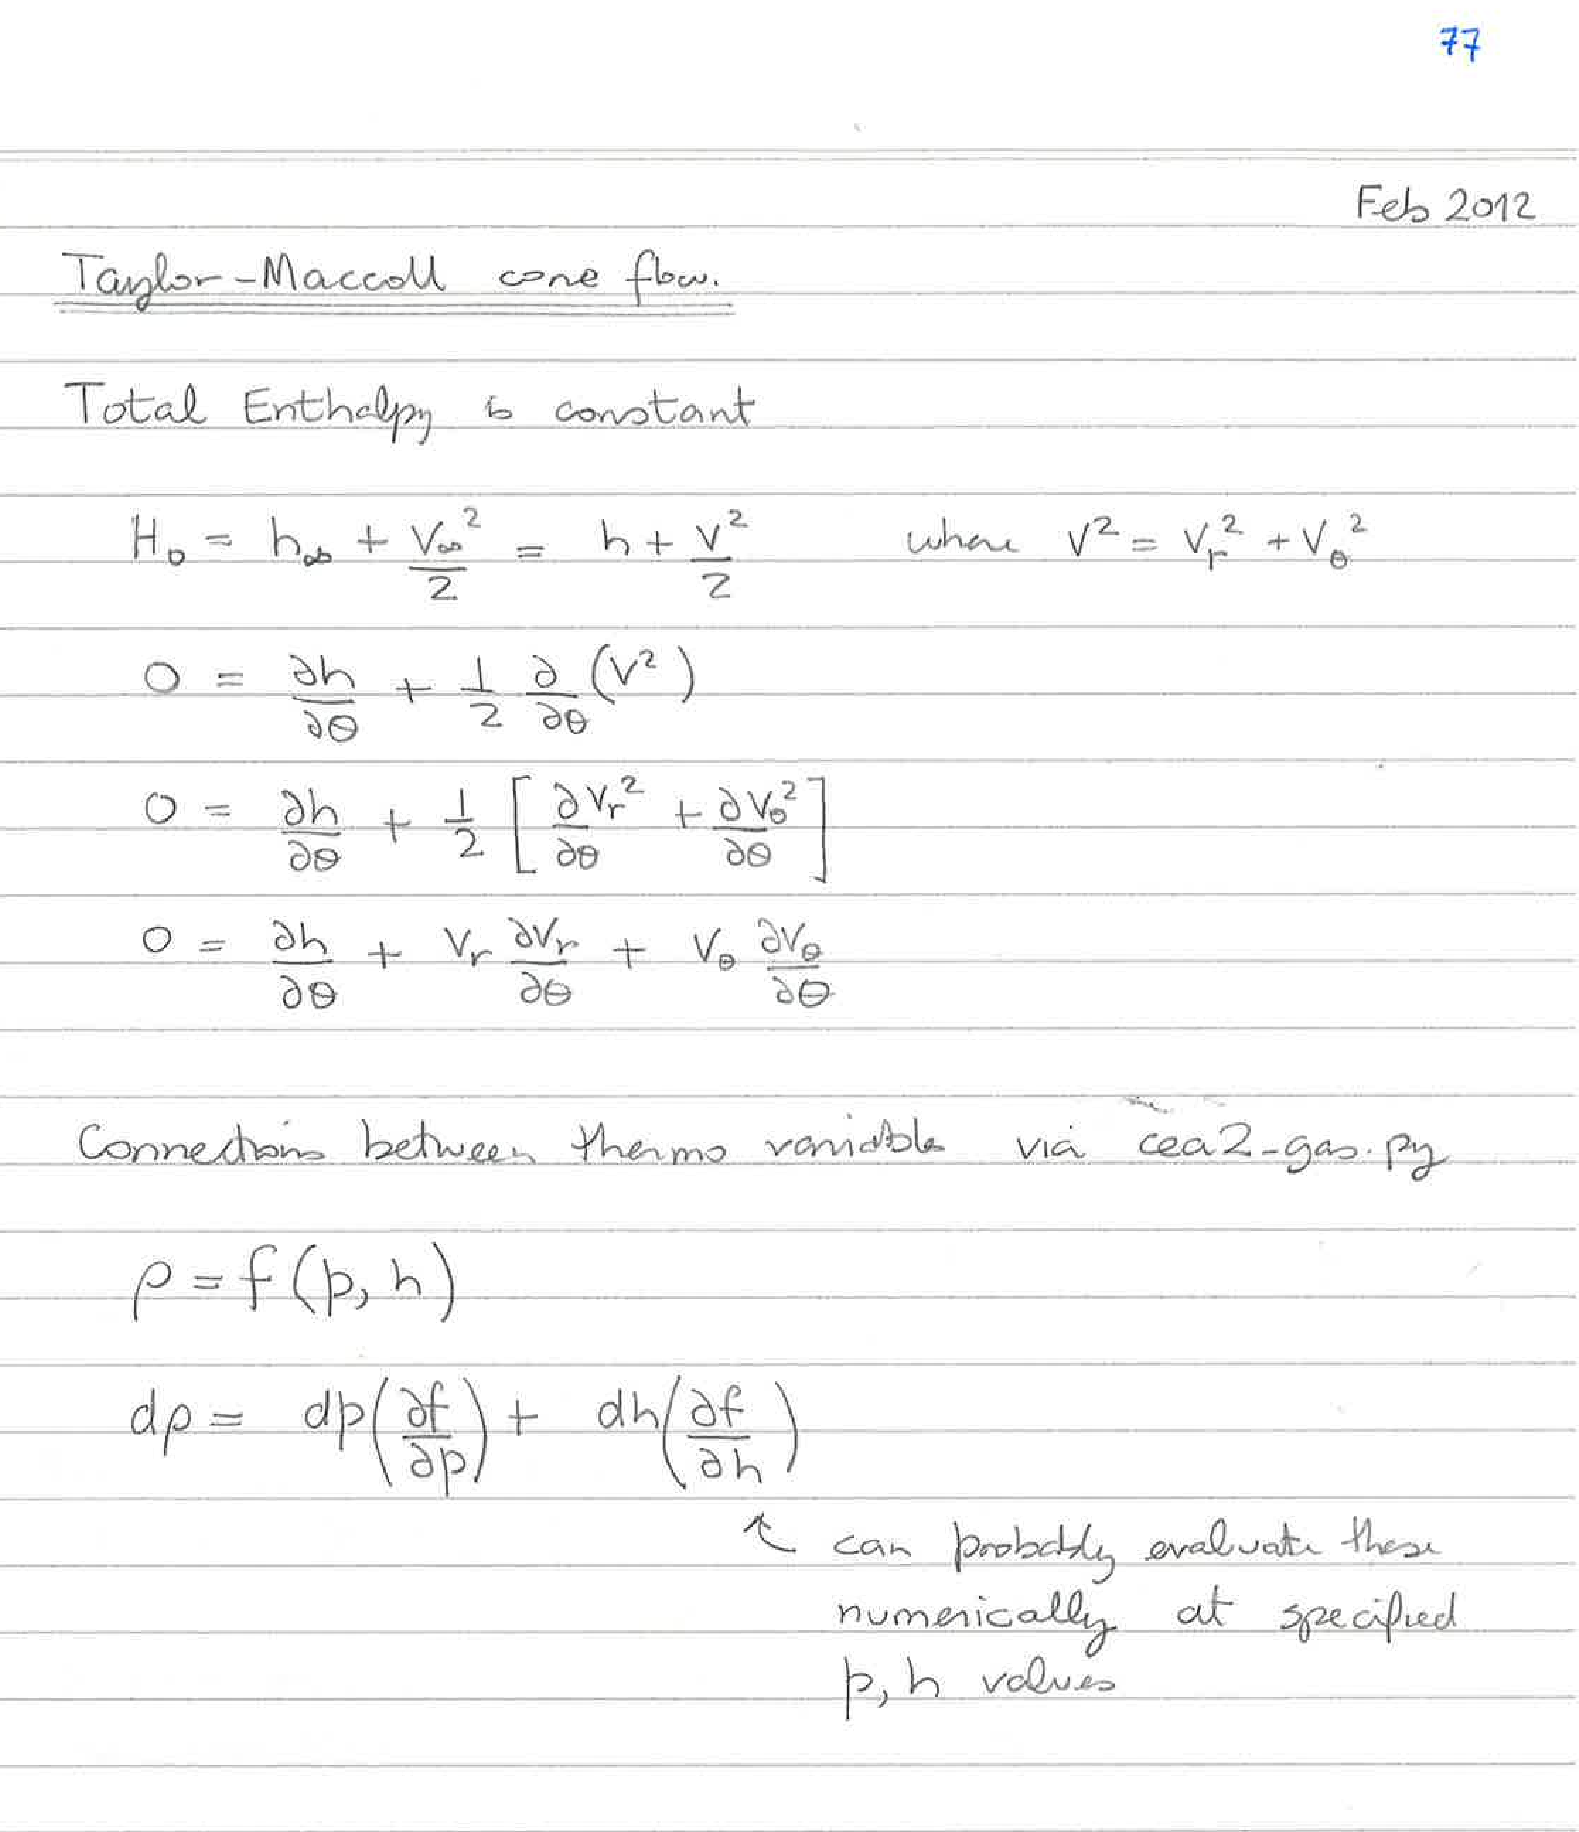
\includegraphics[width=\textheight,angle=90]{../figs/pj-workbook-page-77.png}
\end{center}

\newpage
\begin{center}
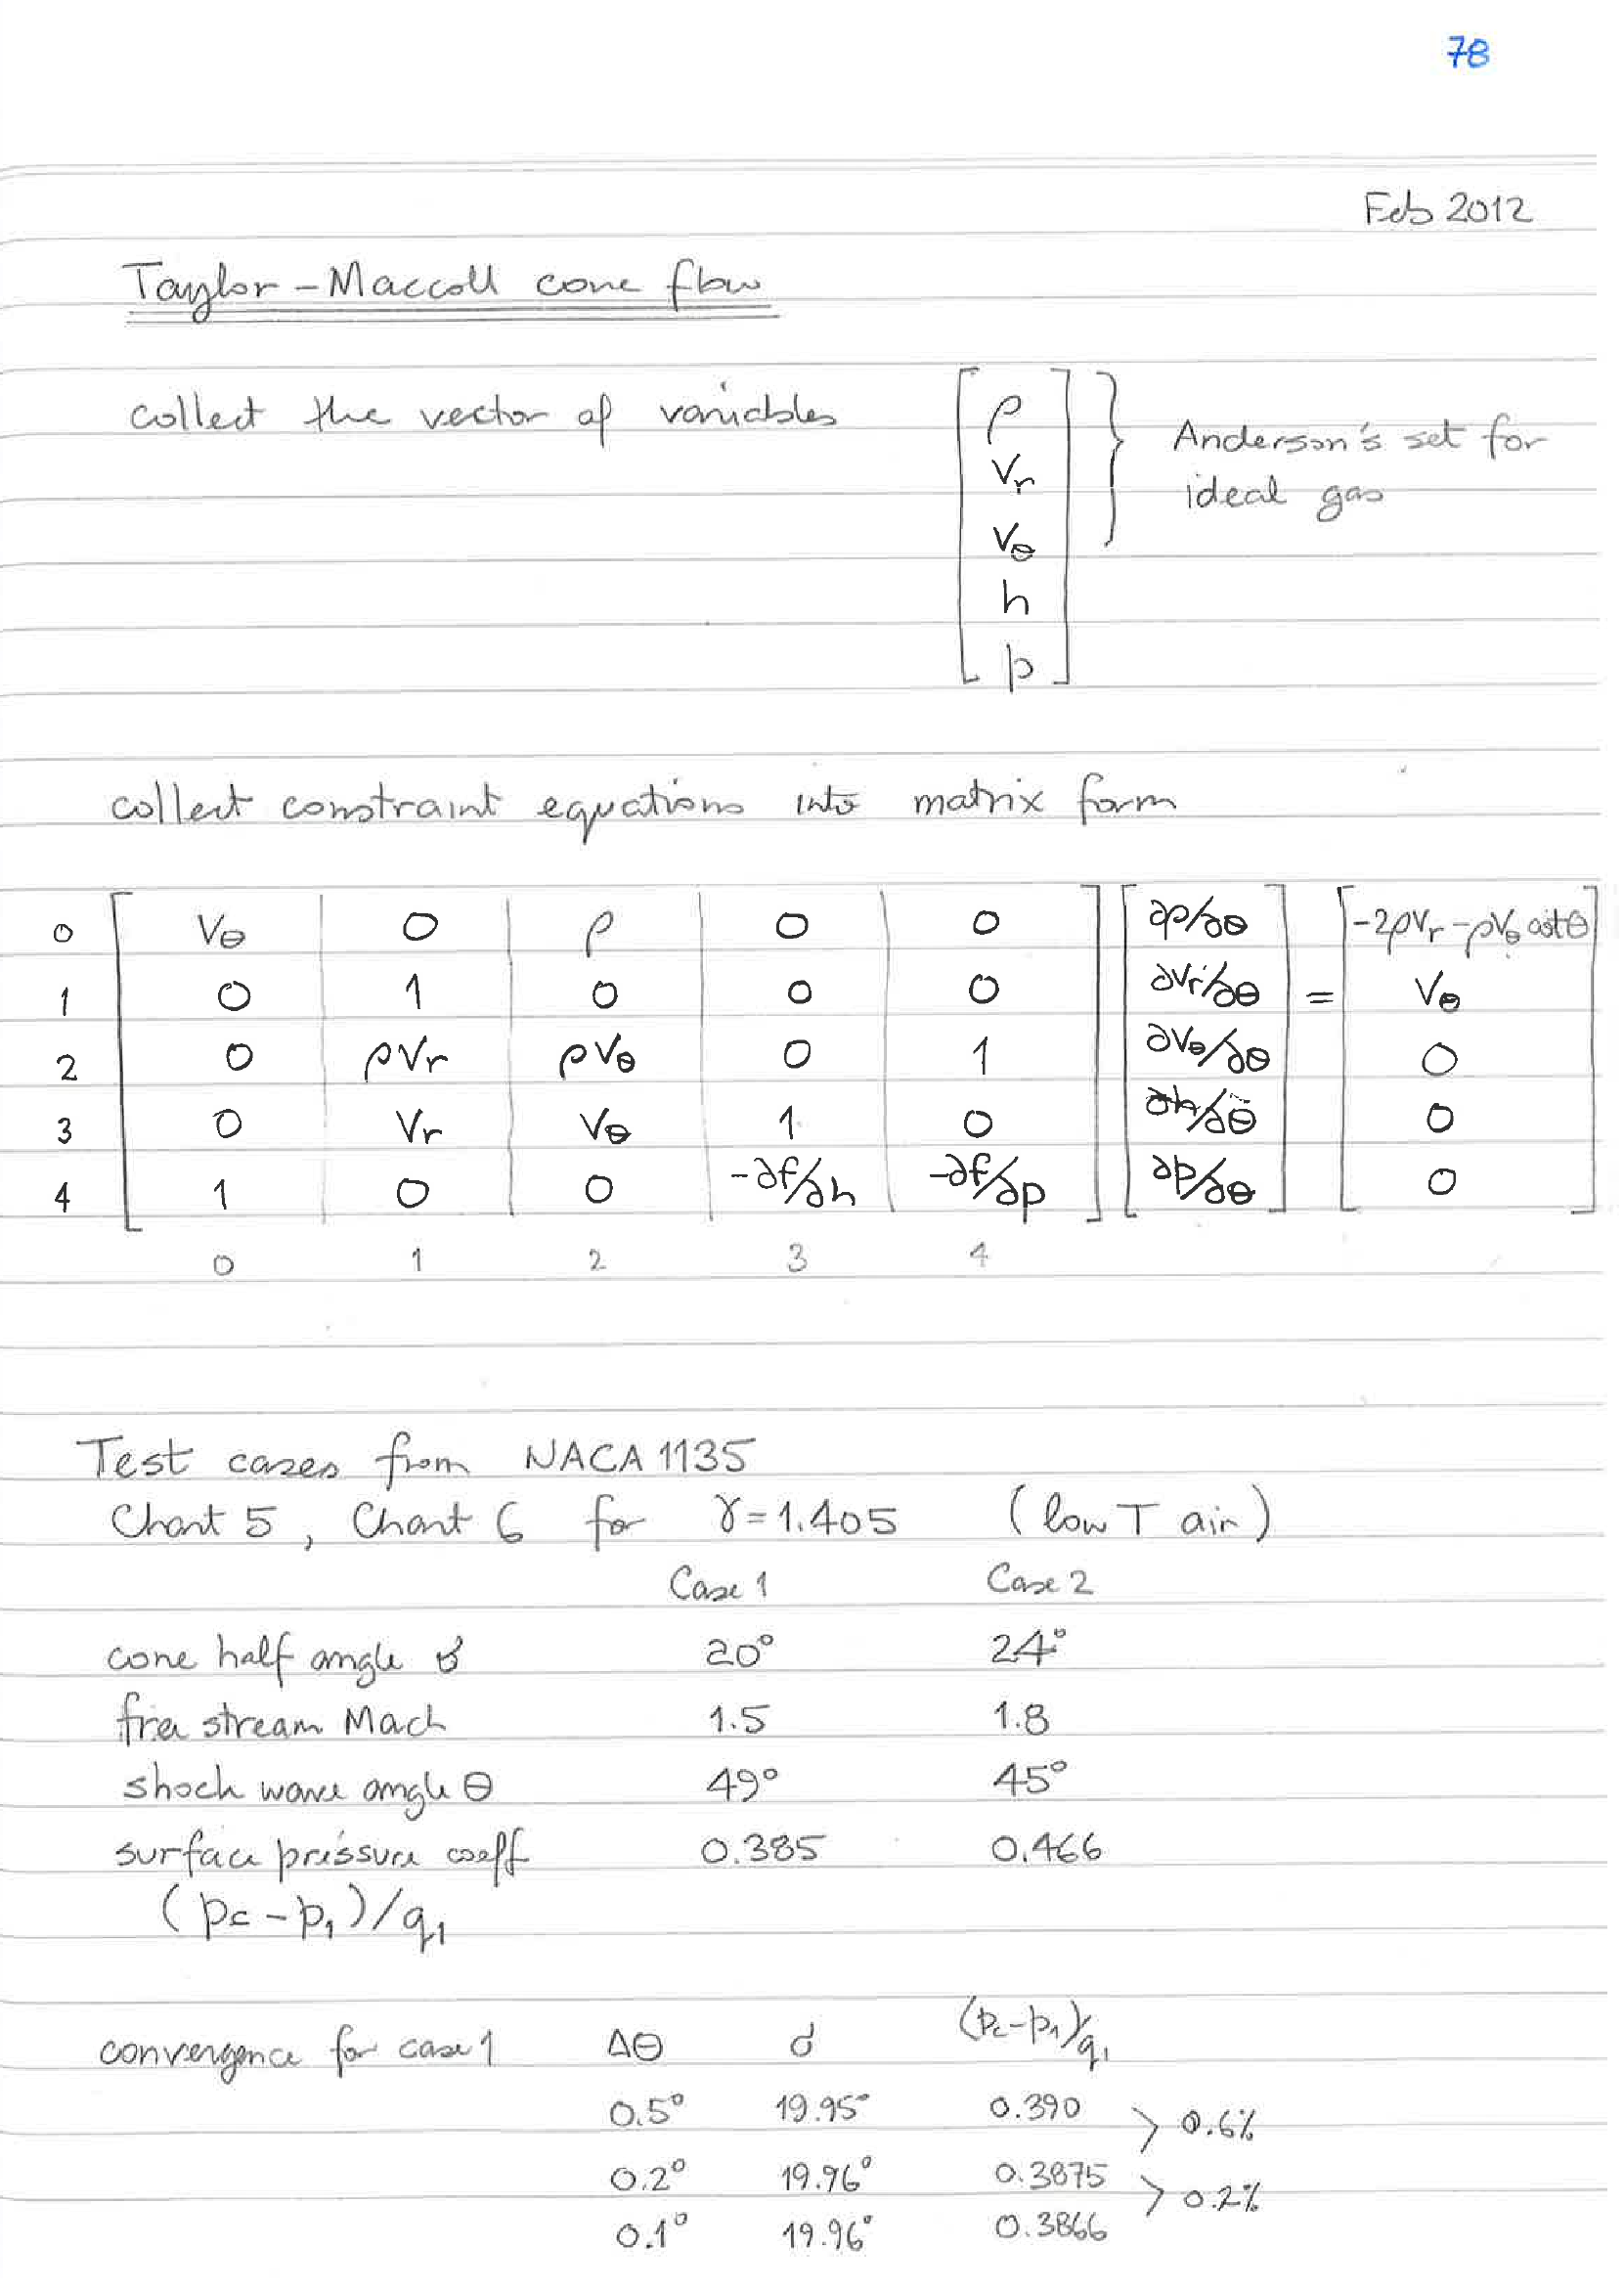
\includegraphics[width=\textheight,angle=90]{../figs/pj-workbook-page-78.png}
\end{center}

\end{document}

